\chapter{Results}
\label{chap:Results}
%importanza loop (cambio stato), confronto a cambio di loop
%discutere i loops e i vari risultati
%noi non prendiamo codici di errorere, ma solo coverage
%punti di forza e debolezza di fallaway
%aflnet e chatafl quasi lineare
%fallaway ha un andamento a scalini, piu' casuale
After 24h of fuzzing, we can look at the results and analyze them.
\section{Fuzzer Analysis}

\subsection{Fallaway}

\begin{itemize}
    \item \textbf{Complete Coverage}: 6\% (883/15168)
    \item \textbf{Total Executions}: 79,987,763
\end{itemize}

\textbf{Strengths:}
\begin{itemize}
    \item \textit{High Execution Count}: Fallaway has a significantly higher number of total executions compared to AFLNet and ChatAFL, indicating its capability to generate and execute a large number of test cases. This increases the likelihood of discovering bugs or vulnerabilities through extensive input space exploration.
    \item \textit{High Code Coverage}: Achieves the highest code coverage among the three fuzzers (6\%), suggesting its strategy is effective at exploring various parts of the code.
\end{itemize}

\textbf{Weaknesses:}
\begin{itemize}
    \item \textit{Efficiency Concerns}: The large number of total executions (nearly 80 million) suggests that Fallaway may be less efficient, requiring more attempts to cover similar amounts of code compared to AFLNet and ChatAFL.
    \item \textit{Potential for Resource Consumption}: The high number of executions may lead to greater consumption of computational resources, which could be a limitation in resource-constrained environments.
\end{itemize}

\textbf{Peculiarities:}
\begin{itemize}
    \item Fallaway’s high execution count aligns with a strategy that relies on brute force to uncover edge cases, which can be effective but may lack sophistication in targeting specific code paths.
\end{itemize}

\subsection{AFLNet}

\begin{itemize}
    \item \textbf{Complete Coverage}: 5\% (830/15168)
    \item \textbf{Total Executions}: 209,776
\end{itemize}

\textbf{Strengths:}
\begin{itemize}
    \item \textit{Efficient Execution}: With the lowest number of total executions (around 210,000), AFLNet is highly efficient in achieving its results. This suggests AFLNet is effective in targeting specific code parts with minimal test cases, leveraging coverage-guided strategies.
    \item \textit{Specialization in Network Protocols}: Optimized for fuzzing network protocols, AFLNet is particularly effective in testing stateful communications and complex protocol interactions.
\end{itemize}

\textbf{Weaknesses:}
\begin{itemize}
    \item \textit{Lower Code Coverage}: AFLNet achieves slightly lower coverage (5\%) compared to Fallaway and ChatAFL, indicating it might not explore as many diverse code paths outside of network protocol contexts.
    \item \textit{Limited in Broader Contexts}: Its specialization in network protocols may limit its effectiveness for fuzzing applications that do not primarily involve network communication.
\end{itemize}

\textbf{Peculiarities:}
\begin{itemize}
    \item AFLNet's use of network-specific heuristics allows it to focus on relevant test cases, leading to fewer, more meaningful executions, but potentially missing general-purpose vulnerabilities.
\end{itemize}
\phantom{}\\
\subsection{ChatAFL}

\begin{itemize}
    \item \textbf{Complete Coverage}: 6\% (850/15168)
    \item \textbf{Total Executions}: 241,242
\end{itemize}

\textbf{Strengths:}
\begin{itemize}
    \item \textit{Balanced Approach}: ChatAFL exhibits a balance between execution count and coverage. With a medium number of executions (around 241,000) and competitive code coverage (6\%), it balances efficiency and effectiveness.
    \item \textit{High Coverage with Fewer Executions}: Achieves similar coverage to Fallaway but with significantly fewer executions, indicating a more optimized strategy in selecting test cases.
\end{itemize}

\textbf{Weaknesses:}
\begin{itemize}
    \item \textit{Potential Limitations in General Fuzzing Tasks}: While optimized for certain scenarios, its overall effectiveness may vary depending on the specific use case and target application.
\end{itemize}

\textbf{Peculiarities:}
\begin{itemize}
    \item ChatAFL may use advanced techniques, such as machine learning or heuristics, to improve test case selection, achieving comparable coverage to Fallaway with significantly fewer executions.
\end{itemize}

\section{Coverage Analysis Over Time and Configurations}

The coverage of the three fuzzers over 24h is shown in Figure \ref{fig:coverage_1day}.
\begin{figure}[H]
    \centering
    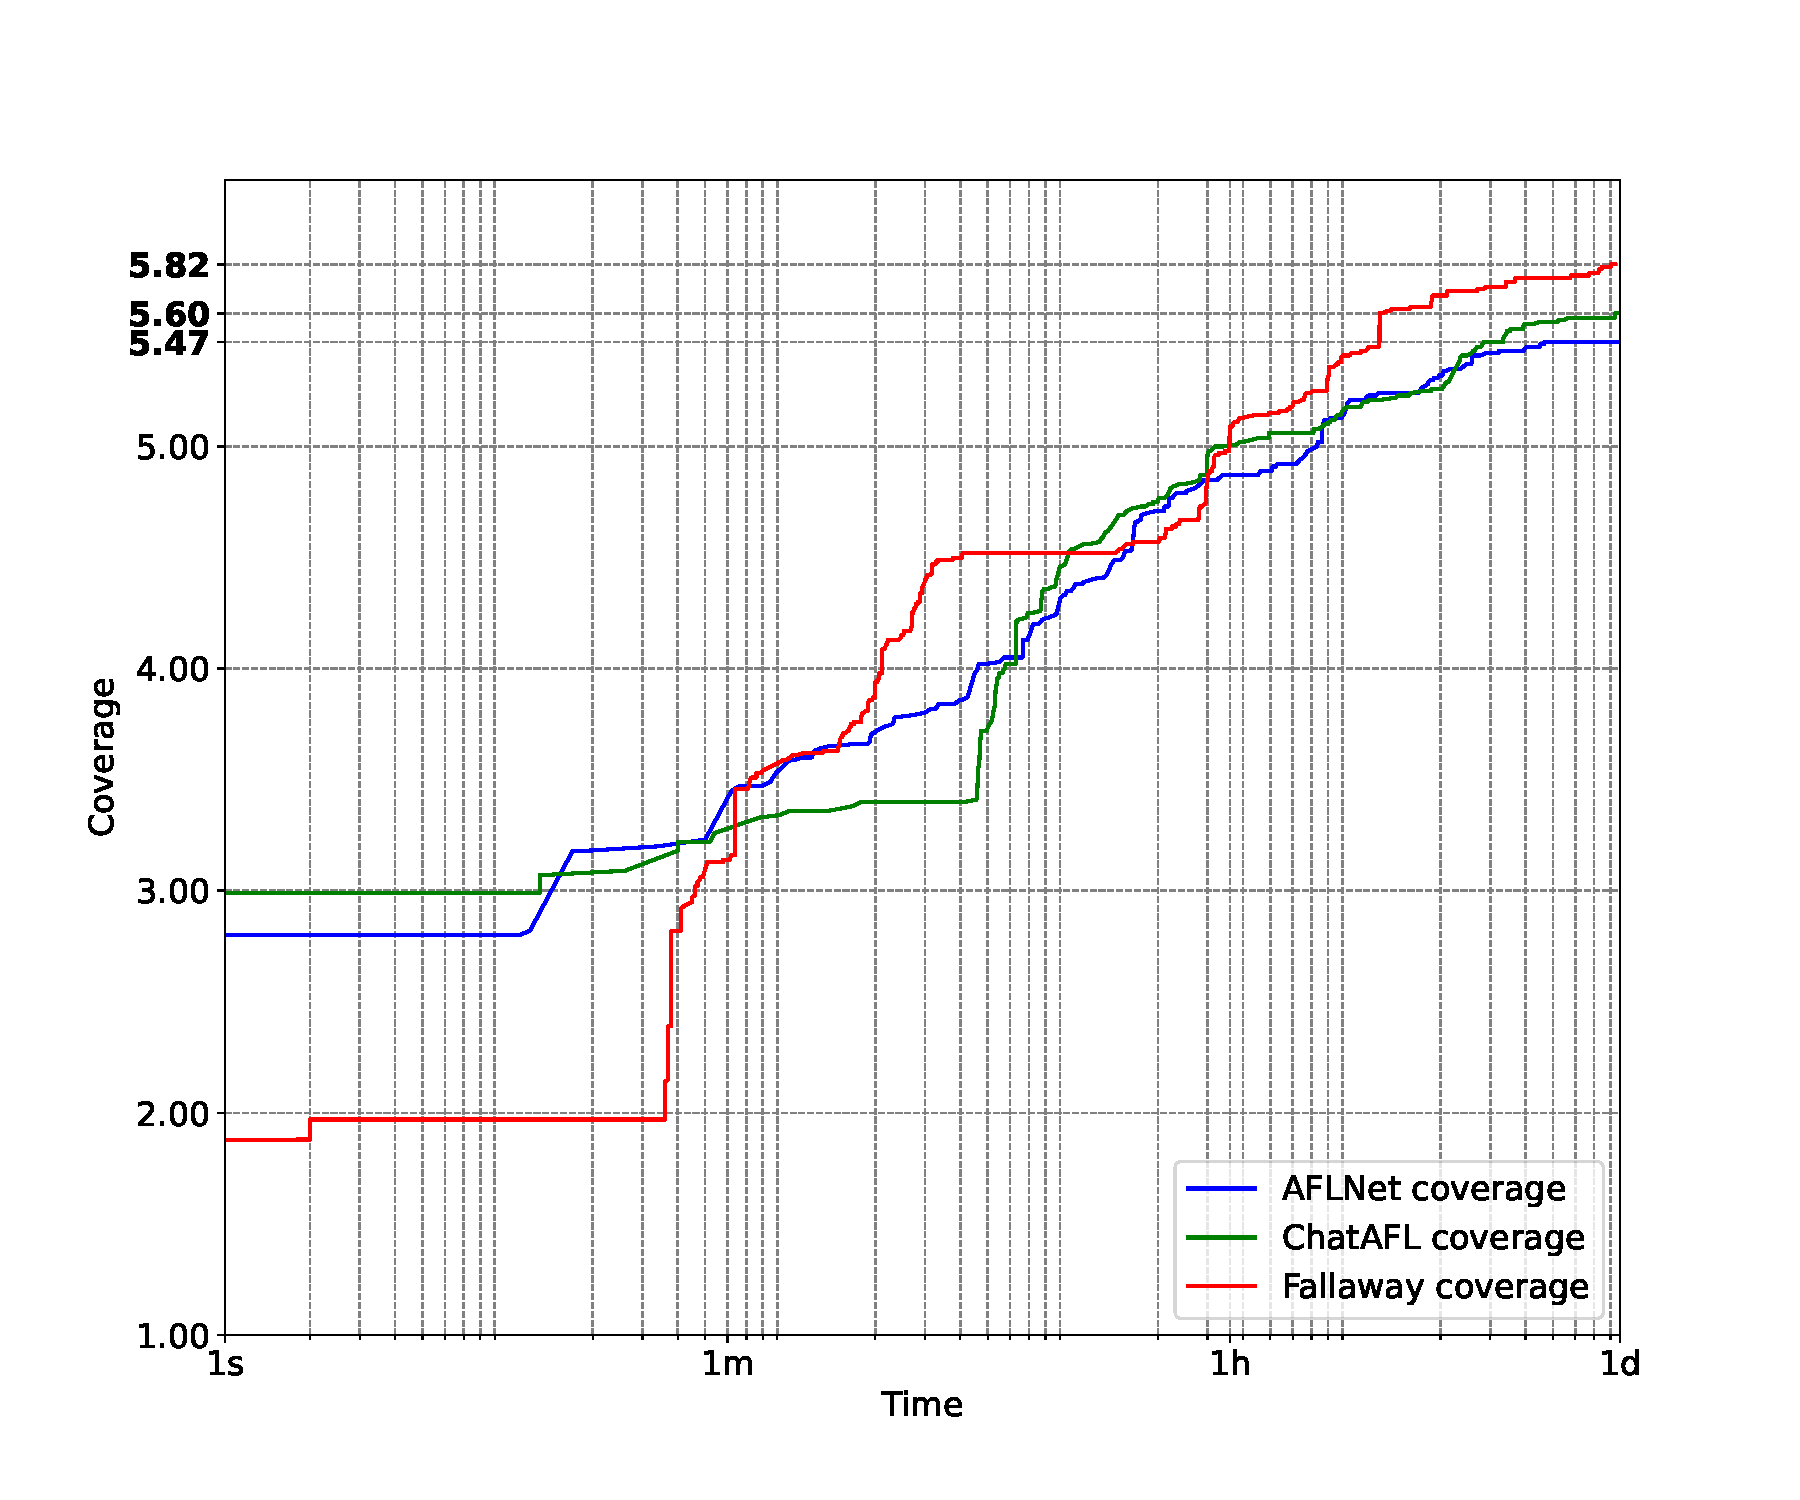
\includegraphics[width=1\textwidth]{Images/coverage_over_time_lighttpd-1day-1000l.pdf}
    \caption{Coverage of the three fuzzers in 24h}
    \label{fig:coverage_1day}
\end{figure}
\phantom{}\\
As we already mentioned, Fallaway hasn't a linear growth in coverage, but it has a more random behavior. This could be due to the state model that we have implemented, which consider only two state for the existence or non-existence of a resource. This could be limiting and could be improved by defining a better state model, adding even more states.
\\AFLNet and ChatAFL have a more linear growth in coverage, which is a good thing because it means that they are more efficient in exploring the code (in fact they starts already from a higher coverage than Fallaway, that means that they are more aimed to explore the code).
\\In another experiment, we ran the fuzzers for 10 hours, modifying the configuration of Fallaway to be in a loop of 250.
\\The coverage of the three fuzzers over 10h is shown in Figure \ref{fig:coverage_10hours}.

\begin{figure}[H]
    \centering
    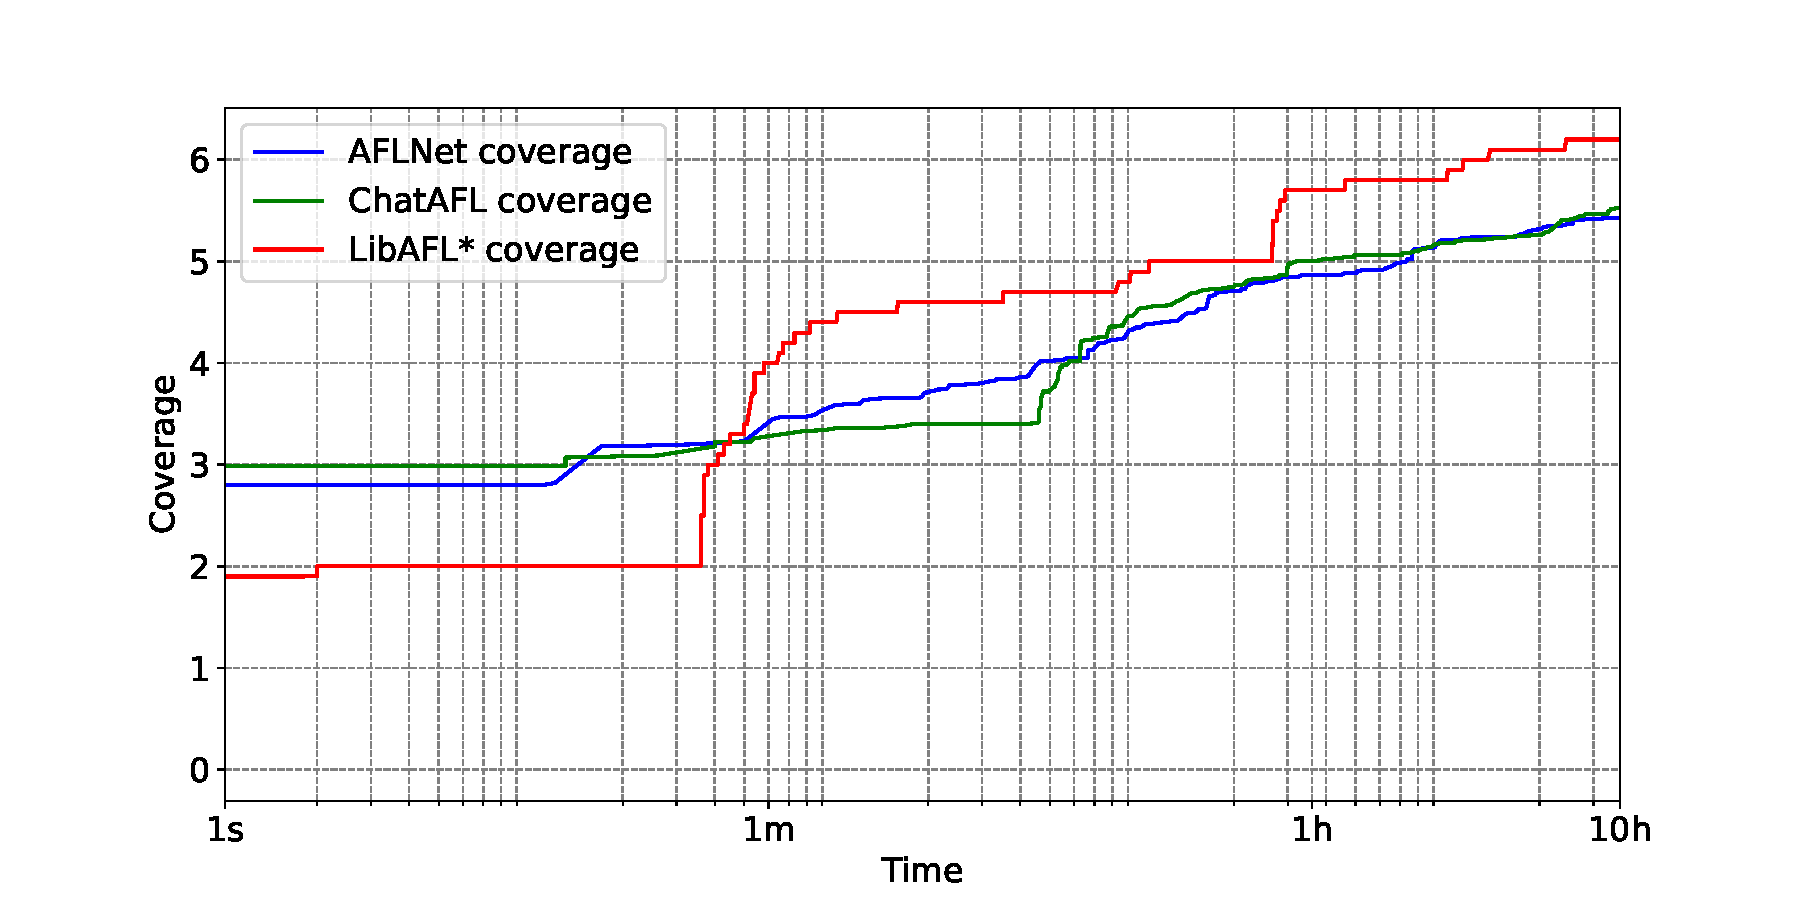
\includegraphics[width=1\textwidth]{Images/coverage_over_time_lighttpd-10h.pdf}
    \caption{Coverage of the three fuzzers in 10 hours}
    \label{fig:coverage_10hours}
\end{figure}
\phantom{}\\
In this configuration, Fallaway has reached a complete\_coverage of 6\% (942/15168).
\\This is 59 more edge cases than the previous configuration, which is a 6.7\% increase.
\\This could be due to the fact that the fuzzer is running in a loop of 250, which allows it to run more test cases in a shorter amount of time.
\\This is not always a good thing, it depends on the SUT, corpus, configurations and more because in general: higher loop values can lead to more coverage, but also to more redundant test cases and to stuck on states that makes low progress; lower loop values can lead to less coverage, but also to less redundant test cases and to faster progress.
